\section{End-to-End Integration with HigherHRNet}
\label{sec_res_e2e}

This section closes the experimental evaluation by replacing the
ground-truth keypoint input used in the preceding COCO experiments with
detections produced by HigherHRNet-W32-512~\cite{cheng2020higherhrnet}.
The resulting evaluation therefore measures PG-GAT under the
end-to-end protocol of Section~\ref{sec_meth_integration},
where the grouping module operates on detected rather than annotated
keypoints.

Two configurations are reported.
In the oracle-$K$ configuration,
the number of people $K$ is taken from the ground-truth annotation,
while the keypoint locations themselves are supplied by HigherHRNet.
This separates the performance of the PG-GAT embedding and $k$-means
read-out from errors in estimating the number of clusters.
In the autonomous configuration,
$K$ is instead predicted by the frozen-backbone K-estimation head
of Section~\ref{sec_meth_kestimation}.
The latter therefore represents the complete operational pipeline -
HigherHRNet detects the keypoints,
PG-GAT embeds them,
the K head estimates the number of people,
and $k$-means produces the final grouping without using ground-truth
information at inference.

\subsection{Setup}
\label{sec_res_e2e_setup}

The detector used for the end-to-end evaluation is
HigherHRNet-W32-512 with COCO-trained weights.
It is held fixed throughout the experiment -
no detector fine-tuning,
head replacement,
or retraining is performed.
HigherHRNet produces a heatmap for each joint type,
from which its internal non-maximum suppression extracts the keypoint
candidates used for grouping.
The same candidate set is provided to HigherHRNet's native
associative-embedding (AE) grouping and to PG-GAT,
ensuring that differences between the two grouping results are not
caused by differences in the detected keypoints.

For evaluation,
detected keypoints are matched to the ground-truth annotations
using a per-joint-type Hungarian assignment with a 10-pixel distance
threshold.
Each successfully matched detection is thereby assigned a ground-truth
person identity,
which is used only to compute the metric.
Unmatched detections are excluded from the PGA calculation,
so the resulting score measures grouping accuracy on the matched
detections rather than keypoint detection recall.
Both AE and PG-GAT are evaluated against this same set of matched
detections.

The PG-GAT model is the \texttt{meng-headline} checkpoint selected in
Section~\ref{sec_res_coco_ft}.
For the oracle-$K$ configuration,
$k$-means uses the ground-truth number of people in the scene.
For the autonomous configuration,
this value is replaced by the output of the frozen-backbone
K-estimation head described in Section~\ref{sec_meth_kestimation},
trained on embeddings from the COCO distribution.
Ground-truth identities attached during Hungarian matching are used
only after grouping to compute PGA
and do not enter the autonomous inference pipeline.

\subsection{Headline numbers}
\label{sec_res_e2e_numbers}

\begin{table}[H]
\centering
\footnotesize
\begin{tabular}{lcl}
\toprule
Configuration & COCO E2E PGA (HigherHRNet detections) & W\&B run \\
\midrule
HigherHRNet AE (native grouping reference)
    & 0.9847 & --- \\
\midrule
PG-GAT + $k$-means (synthetic only)
    & 0.8766 & \texttt{r5ekg0zl} \\
PG-GAT + $k$-means (legacy 20-ep COCO fine-tune)
    & 0.9430 & \texttt{ugzbgepn} \\
PG-GAT + $k$-means (\texttt{meng-headline}, oracle $K$)
    & 0.9591 & \texttt{b5noyg7t} \\
\textbf{PG-GAT + $k$-means (\texttt{meng-headline}, predicted $K$)}
    & \textbf{0.9644} & \texttt{b5noyg7t} \\
\midrule
Hyperbolic PG-GAT, Option~B ($d=32$, COCO fine-tuned)
    & 0.9336 & \texttt{lragtfzu} \\
\bottomrule
\end{tabular}
\caption[End-to-end grouping results on COCO using detections from HigherHRNet-W32-512.]{End-to-end grouping results on COCO using detections from
HigherHRNet-W32-512. HigherHRNet's native associative-embedding
grouping is evaluated on the same matched detections and provides the
detector-specific reference. The \texttt{meng-headline} PG-GAT reaches
$0.9591$ PGA when $k$-means is given the ground-truth person count and
$0.9644$ when the cluster count is supplied by the frozen-backbone
K-estimation head. The latter is the fully autonomous PG-GAT
configuration and requires no ground-truth information at inference.
The remaining gap to HigherHRNet AE is $0.0203$ for the autonomous
configuration.}
\label{tab:e2e_headline}
\end{table}

\subsection{Interpretation}
\label{sec_res_e2e_discussion}

Three observations close the experimental chapter.

\textbf{1. The remaining gap to detector-native grouping is small:}
With the ground-truth person count supplied to $k$-means,
the \texttt{meng-headline} checkpoint reaches an end-to-end PGA of
$0.9591$,
compared with $0.9847$ for HigherHRNet's native AE grouping.
The resulting difference is $0.0256$.

This gap decreases consistently over the course of the investigation.
The synthetic-only two-layer PG-GAT configuration reaches $0.8766$,
leaving a difference of $0.1081$ to the same AE reference.
The synthetic-only architecture-sweep winner reduces this difference
to $0.0842$,
the legacy COCO fine-tune reduces it further to $0.0417$,
and the fine-tune-sweep checkpoint reaches the final oracle-$K$
difference of $0.0256$.
The progression shows that both architecture selection and adaptation
to the COCO distribution contribute to closing the gap to detector-native
grouping.

The $0.0256$ difference should not be interpreted as a direct
measurement of the cost of modularity alone.
HigherHRNet AE and PG-GAT differ in their representation,
training objective,
and access to detector features in addition to whether grouping is
trained jointly with detection.
The result instead measures the remaining empirical gap between
the modular PG-GAT grouping pipeline and the detector's native grouping
mechanism under the evaluation protocol used here.
Section~\ref{sec_disc_embedding_pggat} considers the possible sources
of this difference.

\textbf{2. PG-GAT demonstrates grouping independently of the
detector's grouping mechanism:}
HigherHRNet AE reaches $0.9847$ on the matched detections and provides
the detector-specific reference for this experiment.
PG-GAT reaches $0.9591$ on the same evaluation protocol using
the detector only as a source of keypoint candidates.
It does not consume HigherHRNet's AE tags or internal grouping
assignments,
and the HigherHRNet parameters remain frozen throughout the experiment.

This result demonstrates the practical separation between detection
and grouping that motivates PG-GAT.
Once keypoints and their joint types have been extracted,
grouping is performed by a separately trained embedding network
rather than by a grouping representation learned jointly with the detector.
This differs from architectures in which detection and grouping are
components of the same trained model -
including HigherHRNet AE and other integrated pose-estimation
approaches such as DEKR~\cite{geng2021dekr} and
ED-Pose~\cite{yang2023edpose}.
The detector-swap experiments reported separately provide the stronger
empirical test of whether this separation transfers to detectors other
than HigherHRNet.

\textbf{3. The autonomous pipeline slightly exceeds the oracle-$K$
diagnostic:}
Replacing the ground-truth value of $K$ with the prediction from the
frozen-backbone K head produces the fully autonomous configuration.
HigherHRNet supplies the keypoint candidates,
PG-GAT embeds them,
the K head estimates the cluster count,
and $k$-means produces the final partition.
No ground-truth quantity is required by this sequence at inference.

The autonomous configuration reaches an end-to-end PGA of $0.9644$,
which is $0.0053$ higher than the $0.9591$ obtained when $k$-means is
given the annotation-level person count.
The K head itself achieves $76.1\%$ exact-count accuracy on the COCO
validation set,
rising to $91.9\%$ when predictions within one person of the target
are counted.
Figure~\ref{fig:k_confusion} shows the full distribution of predicted against annotated counts.

\begin{figure}[H]
    \centering
    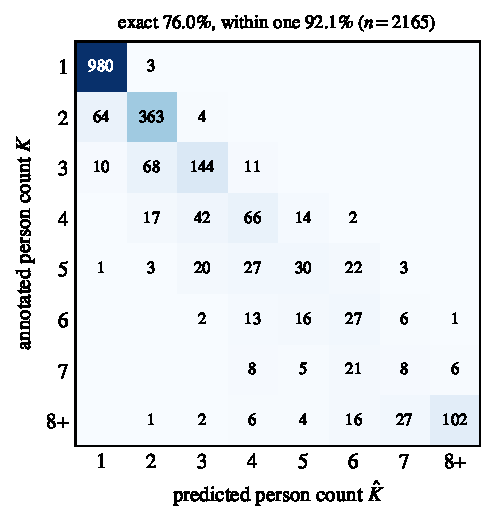
\includegraphics[width=0.64\linewidth]{figures/k_confusion.pdf}
    \caption[Predicted against annotated person count for the K head on HigherHRNet detections.]{Predicted person count $\hat{K}$ from the frozen K head against the annotated count $K$
    on the $2{,}165$ scored HigherHRNet scenes.
    Counts of eight or more are pooled into the last row and column.
    Mass below the diagonal is under-counting.
    The matrix comes from a re-run of the pipeline that reproduces the reported aggregates
    to within $0.0003$ PGA;
    two scenes receive a different count than in the logged run,
    which is why the exact-count rate reads $76.0\%$ here against $76.1\%$ in the text.}
    \label{fig:k_confusion}
\end{figure}

At first sight, a predicted cluster count outperforming the
ground-truth count appears counter-intuitive.
The distinction is that the ground-truth $K$ describes the people
annotated in the image,
whereas $k$-means operates only on the keypoints that survive detection
and matching.
Under the 10-pixel matching threshold,
HigherHRNet recovers $53{,}131$ of $66{,}998$ evaluated ground-truth
keypoints,
corresponding to $79.3\%$ recall.
The graph presented to PG-GAT is therefore an incomplete representation
of the annotated scene.

One plausible explanation for the $0.0053$ improvement is that the
annotation-level $K$ can exceed the number of people that are
meaningfully represented by the detected keypoints in some scenes.
In such cases, forcing $k$-means to use the annotation-level count may
split otherwise coherent detected groups.
The K head instead predicts from the detected embeddings
and can therefore produce a count that is better aligned with the
observed graph.
Confirming this mechanism directly would require comparing $\hat{K}$
with the number of distinct ground-truth identities represented among
the matched detections
rather than with annotation-level $K$ alone.

Regardless of the cause of the small improvement,
the autonomous result establishes the operational result required by
Section~\ref{sec_meth_integration} -
the complete pipeline can produce person-grouped keypoints without
using ground-truth information at inference.
Its PGA of $0.9644$ leaves a difference of $0.0203$ to HigherHRNet's
native AE grouping on the same evaluation protocol
and is the final autonomous result of the experimental investigation.
Figure~\ref{fig:e2e_examples} shows the three groupings on four scored scenes.

\begin{figure}[H]
    \centering
    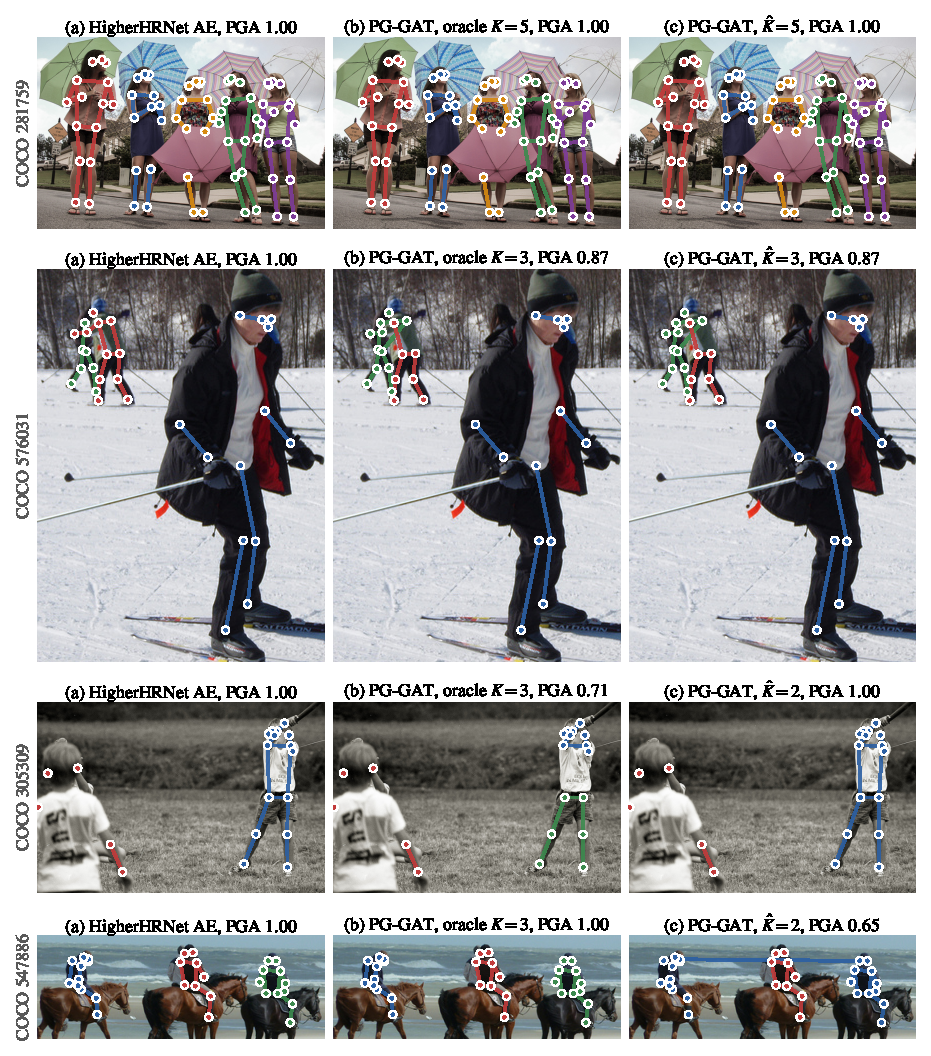
\includegraphics[width=0.97\linewidth]{figures/e2e_examples.pdf}
    \caption[Four scored COCO scenes under the three end-to-end groupings.]{Four scored COCO \texttt{val2017} scenes under the end-to-end protocol:
    (a) HigherHRNet's native AE grouping,
    (b) PG-GAT with $k$-means at the annotated $K$,
    and (c) PG-GAT with the K head's $\hat{K}$.
    Only the detections matched to ground truth are drawn,
    coloured by the person their cluster is assigned to under Hungarian matching,
    so a joint in another person's colour is a grouping error -
    the PGA in each title is the per-scene value.
    From the top: five people grouped correctly by all three;
    a grouping error at the correct count;
    a third annotated person with no matched detections,
    so the annotated $K$ splits a person while the K head's $\hat{K}=2$ does not;
    and an under-count that merges two people.}
    \label{fig:e2e_examples}
\end{figure}

\subsection{Relationship between PGA and AP@OKS}
\label{sec_res_e2e_ap}

The grouping baselines reviewed in Chapter~\ref{chap_2} are primarily
reported using AP under the OKS threshold family,
whereas the results in this chapter use PGA.
The two metrics evaluate different parts of the pose-estimation problem,
and their numerical values are therefore not directly comparable.

AP@OKS evaluates the complete pose-estimation pipeline.
A predicted person instance receives credit according to the similarity
between its assembled keypoints and a ground-truth pose under the OKS
criterion.
Detection failures,
keypoint localisation errors,
and incorrect grouping can therefore all reduce AP.
PGA instead conditions on the set of detections that have already been
matched to ground-truth keypoints
and evaluates whether those detections are assigned to the correct
person (Section~\ref{sec_meth_integration_e2e_metric}).
It consequently removes detection recall and localisation error from
the quantity being measured
and isolates the grouping decision more directly.

Grouping errors also affect the two metrics differently.
Under PGA, an incorrectly grouped keypoint contributes directly
as an incorrect assignment.
Under AP@OKS, the effect depends on how that error changes the
assembled person instances.
For example, exchanging keypoints between two people can reduce
the OKS of both predicted poses
and may therefore affect the AP contribution of both instances.
A fixed change in PGA consequently has no fixed numerical correspondence
to a change in AP@OKS.

HigherHRNet provides a useful reference between the two evaluation
views.
For the W32-512 configuration,
HigherHRNet reports an AP of $0.671$ on COCO \texttt{val2017} under its
published single-scale evaluation with flip testing~\cite{cheng2020higherhrnet},
while its native AE grouping reaches $0.9847$ PGA under the
matched-detection protocol used in this work.
These values should not be interpreted as a formal decomposition of AP,
since the metrics and evaluation procedures differ.
They nevertheless show that, once HigherHRNet keypoints have been
successfully detected and matched, its native grouping mechanism makes
relatively few person-assignment errors.
The substantially lower end-to-end AP must therefore reflect error
sources that PGA intentionally excludes,
in addition to any grouping errors that remain.

This distinction explains the use of PGA as the primary metric in the
present investigation.
PG-GAT replaces the grouping stage rather than the upstream keypoint
detector,
so PGA measures the component of the pipeline that the proposed method
is designed to change.
Reporting AP@OKS for the complete modular system would still be useful
as a system-level evaluation,
but changes in that metric would combine PG-GAT's grouping behaviour
with detection and localisation errors inherited unchanged from the
upstream detector.
PGA is therefore used to isolate the contribution of the grouping method,
while AP@OKS remains the appropriate metric for comparison of complete
pose-estimation systems.

\subsection{Detector-swap evaluation}
\label{sec_res_e2e_swap}

This section reports the detector-swap experiment of
Section~\ref{sec_meth_integration_swap}.
The same frozen \texttt{meng-headline} checkpoint and frozen K head
are applied zero-shot to detections from two additional pose detectors
belonging to different architectural families.
Neither detector contributed training examples to PG-GAT
or to the K-estimation head.

\begin{table}[H]
\centering
\footnotesize
\begin{tabular}{lccccc}
\toprule
Detector (family) & Recall & Native & PG-GAT (oracle $K$) &
PG-GAT (pred.\ $K$) & Gap \\
\midrule
HigherHRNet-W32-512 (heatmap $+$ AE)
    & 0.793 & 0.9847 & 0.9591 & 0.9644 & 0.0203 \\
YOLO11x-pose (single-stage regression)
    & 0.816 & 0.9863 & 0.9647 & 0.9653 & 0.0210 \\
RTMO-L (one-stage bottom-up)
    & 0.774 & 0.9961 & 0.9437 & 0.9741 & 0.0220 \\
\bottomrule
\end{tabular}
\caption[Detector-swap results on COCO \texttt{val2017}.]{Detector-swap results on COCO \texttt{val2017}. Native
denotes each detector's original person assignment evaluated on its
matched-detection subset. The PG-GAT columns discard these assignments,
pool the detected keypoints,
and re-group them using the same frozen \texttt{meng-headline} checkpoint,
with $K$ either taken from the ground truth or predicted by the frozen
K head. Gap is the difference between native grouping and autonomous
predicted-$K$ PG-GAT. The matched subsets contain $2{,}165$,
$2{,}196$, and $2{,}121$ scored images for HigherHRNet,
YOLO11x-pose, and RTMO-L respectively.
Consequently, comparisons between native and PG-GAT are matched within
each detector row, while absolute PGA values should be compared across
detectors with caution. The RTMO native reference uses the publicly
released multi-dataset \texttt{body7} weights.}
\label{tab:e2e_detector_swap}
\end{table}

Two findings follow from Table~\ref{tab:e2e_detector_swap}.

\textbf{1. The gap to detector-native grouping is stable across
detector families:}
The autonomous PG-GAT pipeline trails each detector's native grouping
by $0.0203$,
$0.0210$, and $0.0220$ PGA for HigherHRNet,
YOLO11x-pose, and RTMO-L respectively.
The spread between these three gaps is only $0.0017$ -
despite substantial differences in how the detectors produce and group
their keypoints.

This result provides the direct empirical test of the detector-swap
claim introduced in Section~\ref{sec_meth_integration_swap}.
PG-GAT and the K head are unchanged between all three evaluations
and operate only on the pooled keypoint coordinates,
joint types,
and associated input features.
In particular, neither component is retrained or adapted to
YOLO11x-pose or RTMO-L.
The fact that the autonomous pipeline remains within approximately
$0.02$ PGA of native grouping across all three detectors shows that
its performance is not specific to the HigherHRNet candidate
distribution on which the original end-to-end evaluation was performed.

The gap should not be interpreted as a direct numerical measurement
of the cost of modularity alone.
Each native grouping mechanism differs from PG-GAT in its representation,
training data,
objective,
and access to detector-internal features.
What the experiment establishes is that replacing these detector-specific
assignments with the same external grouping module incurs a small,
and remarkably consistent, empirical gap across the three detector
families tested.
For YOLO11x-pose and RTMO-L, the native person assignment is also
produced as part of the detector itself rather than by a detachable
grouping module.
PG-GAT therefore provides a form of interchangeability that the native
assignments do not.

\textbf{2. The behaviour of predicted $K$ is consistent with an
effective-person-count effect:}
The difference between predicted-$K$ and oracle-$K$ PG-GAT changes
substantially with the detector.
For YOLO11x-pose, which has the highest matched-keypoint recall
at $0.816$, predicted $K$ changes PGA by only $+0.0006$.
For HigherHRNet at $0.793$ recall, the difference increases to
$+0.0053$, while for RTMO-L at $0.774$ recall it reaches $+0.0304$.
In the ground-truth-keypoint evaluation, where the input contains
the annotated keypoints rather than an incomplete detector output,
predicted $K$ instead trails the true count by $0.0066$.

These four operating points form a monotonic pattern -
as the keypoint set becomes less complete,
the annotation-level person count becomes less useful as the cluster
count for the graph actually presented to PG-GAT,
while the count estimated from that graph becomes relatively more useful.
This behaviour is consistent with the explanation proposed in the
HigherHRNet experiment.
If some annotated people are only weakly represented among the surviving
detections, forcing $k$-means to use the annotation-level $K$ can
introduce unnecessary clusters and split otherwise coherent detected groups.
The K head, which predicts from the observed embeddings, can instead
return a count closer to the number of people represented strongly
enough to support grouping.

The detector swap strengthens this interpretation because the same
trend appears across three independently generated detection sets
and reverses in the ground-truth-keypoint control.
It does not, however, prove that recall alone causes the effect -
detector identity,
visibility patterns,
localisation errors,
and the distribution of missing joints also change between the three rows.
A direct test would compare both $K$ and $\hat{K}$ with the number
of distinct ground-truth identities represented by the matched
detections in each scene.
The present result is therefore evidence consistent with the
effective-person-count explanation
rather than a causal isolation of that mechanism.